\chapter{Theoretic Frameworks}
General complexity frameworks for general theoretic areas.


%---------------------------------------------------
%---------------------------------------------------
\section{Meta-complexity}
Some classical problems that are usually reduced to.
%---------------------------------------------------
\subsection{Communication complexity}
\subsubsection{Gap-Hamming-Distance problem}
\begin{prob}[Gap-Hamming\cite{mmmw21}]
\label{ghd}
     Let Alice and Bob be communicating parties who hold vectors $s\in\{\pm1\}^n$ and $t\in\{\pm1\}^n$, respectively. The Gap-Hamming problem asks Alice and Bob to return
     \begin{align*}
         1~if~\langle s,t \rangle\ge \sqrt{n}~~~~~~and~~~~~~-1~if~\langle s,t \rangle\le -\sqrt{n}.
     \end{align*}
     Denote it by $GHD_{n}(x,y)$.
\end{prob}



In general, we need to compute the function $f(x,y)$ for $x\in \mc X, y\in\mc Y$, where $\mc X$ and $\mc Y$ are separate sources and we cannot simultaneously obtain both $x$ and $y$. Instead, we repeatedly communicate information from $x$ to $y$ or from $y$ to $x$, accumulating intermediate information during this process. Finally, we use this accumulative intermediate information to compute $f(x,y)$. The goal is to minimize the number of times of communication or the total amount of communication bits.

To formalize this communication process, a binary tree structure called a "protocol tree" $T$(Fig.\ref{proto_tree}) is used. Each possible value of $f(x,y)$ corresponds to a leaf node $L$ in $T$. The communication complexity is measured by the height $H(T)$ of the tree $T$. Notably, for any node $N$ in $T$, the set $R(N):={(x,y):(x,y)\text{ can reach node $N$}}$ always forms a square, i.e., $R(N)=A\times B$ for some $A\subseteq\mc X$ and $B\subseteq\mc Y$. As a result, the leaf nodes form a rectangular partition of $\mc X\times\mc Y$.

\begin{figure}
  \centering
  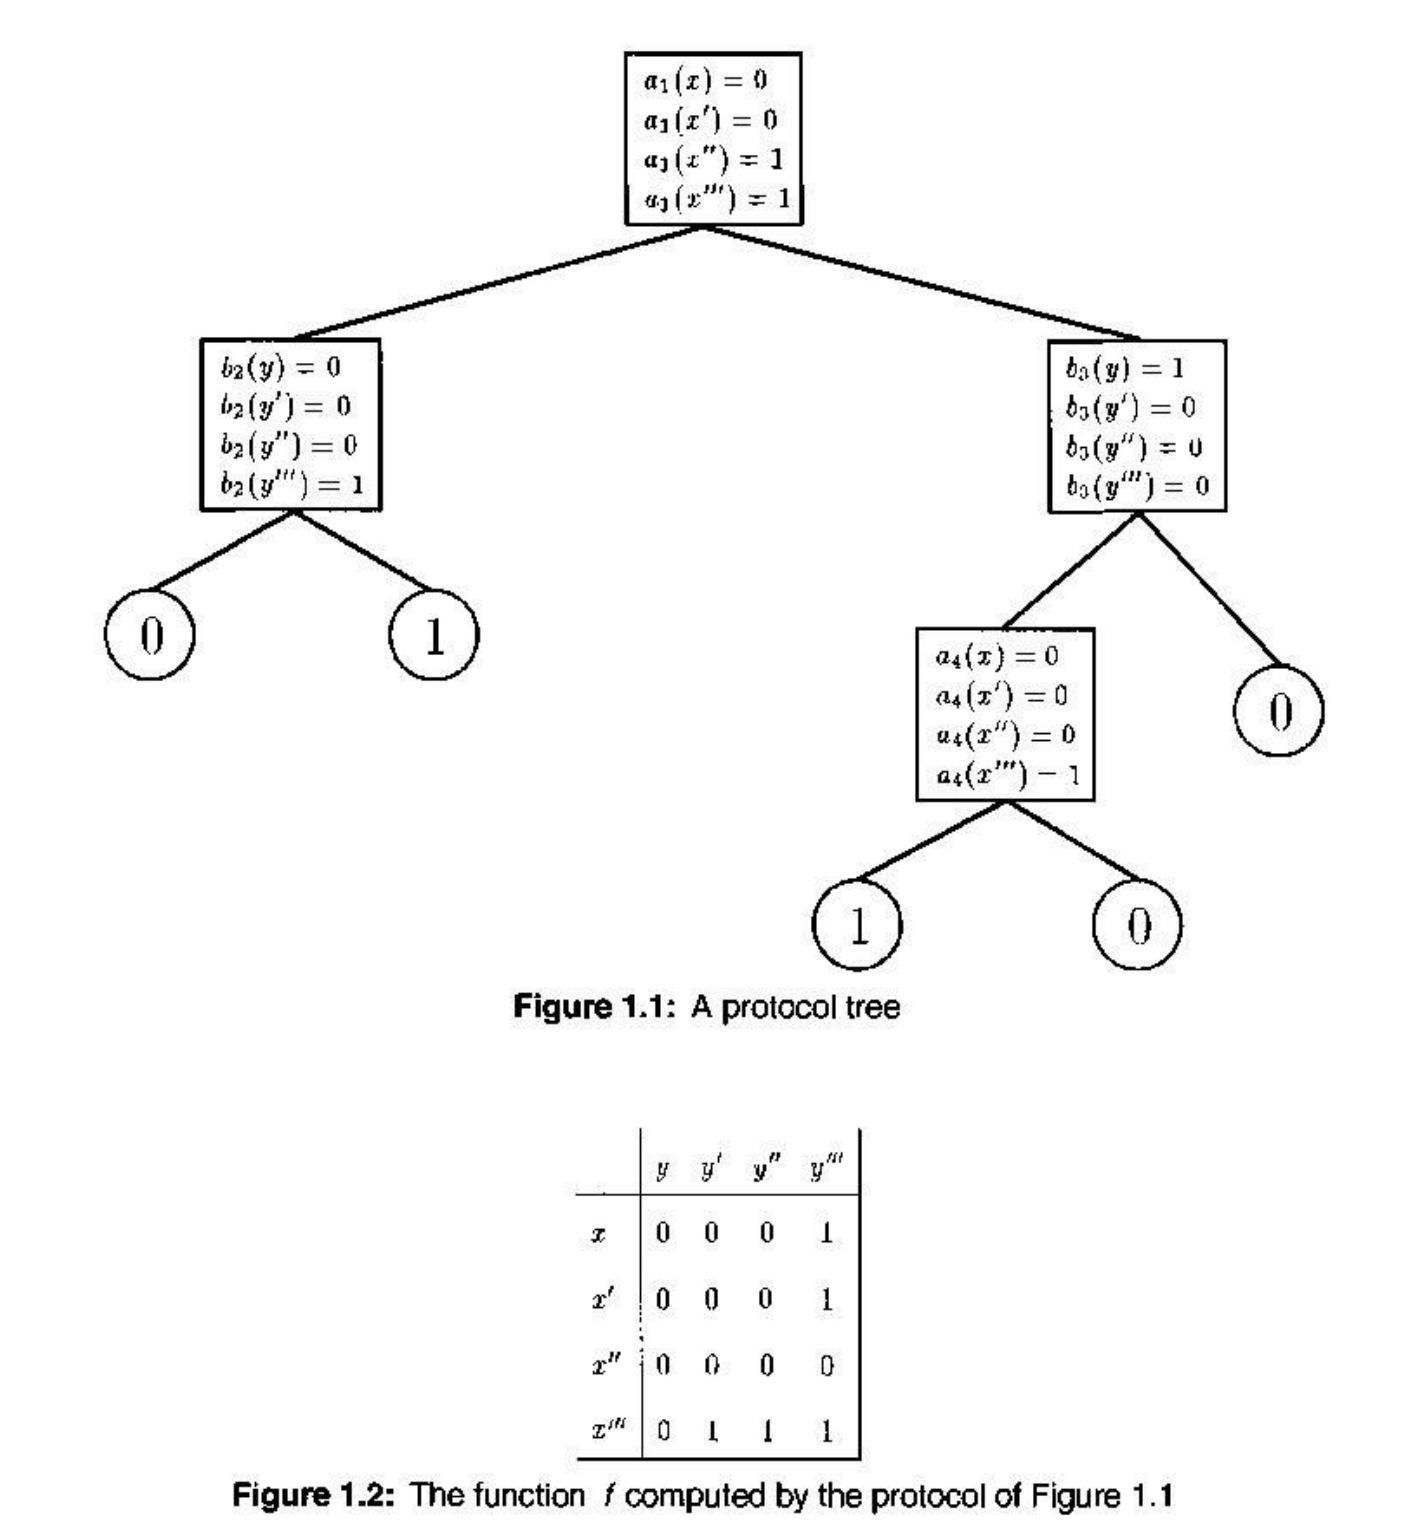
\includegraphics[width=0.5\textwidth]{protocol_tree.png}
  \caption{Protocol tree\cite{kushilevitz1997communication}}
  \label{proto_tree}
\end{figure}

By using the minimum number of square partitions $M_f$ of the function $f(x,y)$, we can derive a lower bound on the communication complexity:

\[
H(T)\ge \log_2 M_f.
\]


\begin{thm}[\cite{cr12}\cite{vidick2012concentration}\cite{sherstov2012communication}]
\label{ghd_lower_bound}
    Any randomized protocol solving problem \ref{ghd} $GHD_n$ with probability $2/3$ needs at least $\Omega(n)$ bits of communication.
\end{thm}

\pfsk{\ref{ghd_lower_bound}}{
The original proof is in \cite{cr12} and \cite{vidick2012concentration} make a simpler one. Here we use proof in \cite{sherstov2012communication}, which is simplist among them.

First, use \textbf{Yao's principle}(theorem \ref{yaoprin}) to reduce the randomness of algorithm to randomness of a distribution $\mu$ of input $(x,y)$. Formally, consider all those deterministic protocol tree $T(x,y)$ such that $\mb P_{(x,y)\sim\mu}[T(x,y)\neq f(x,y)]\le\epsilon$. Denote the minimum complexity(tree height) of such deterministic $T$ by $R_{\mu,\epsilon}(f)$, and denote minimum expectation complexity of random tree with error $\epsilon$ by $C_\epsilon(f)$, we have $C_\epsilon(f)\gtrsim R_{\mu,\epsilon}(f)$. See \cite{yao83} lemma 2 in sect. 3.3 for details.

Then, it suffices to find a hard distribution $\mu$ of $(x,y)$ and lower bound of $R_{\mu,\epsilon}(f)$.
This is done by a trick called \textbf{$\epsilon$-corruption bound}:
\begin{lem}[Yao's corruption bound\cite{sherstov2012communication}]
If $\exists \varepsilon, \delta \in(0,1)$ such that $\mu$ satisfies
$$\mu\left(R \cap f^{-1}(+1)\right)>\varepsilon \mu\left(R \cap f^{-1}(-1)\right)$$
for every rectangle $R \subseteq X \times Y$ with $\mu(R)>\delta$, 
 then $R_{\mu,\xi}(f)\ge\log_2\bbr{\frac{1}{\delta}\left(\mu\left(f^{-1}(-1)\right)-\frac{\xi}{\varepsilon}\right)}$ for small $\xi>0$.
\end{lem}
\noindent Intuitively, the misclassification error in any large rectangle is not so large. Therefore, when total error is a given constant, we can lower bound the number of rectangle partition and thus lower bound the tree height. See \cite{yao83} lemma 3 in sect. 3.3 for originality and details. Usually, people try to directly prove corruption bound for uniformly distribution.

Finally, in our setting, the Gap-Hamming distance problem($GHD_n$) is further reduce to Gap-orthogonality problem($ORT_n$, problem \ref{ort_prob}) with $R_{1/3}(GHD_n)=\Omega(R_{1/3}(ORT_n))$, where $f(x,y)=(-1)\mf 1_{|\langle x,y \rangle|\le\sqrt{n}}+(+1)\mf 1_{|\langle x,y \rangle|\ge2\sqrt{n}}$. 
Note that $f^{-1}(+1)=\{(x,y)||\langle x,y \rangle|\ge2\sqrt{n}\}$, thus the corruption bound intuitively(not so rigorously) means for rectangle $R$ with large probability, we have
\begin{equation}
    \label{anti_concen_ghd}
    \exists c,C>0,~~\mb P_{(x,y)\sim Unif[R]}[|\langle x,y \rangle|>C]\ge c,
\end{equation}
which is essentially a \textbf{anti-concentration analysis}. Choosing uniform distribution is enough, it is proved by \textbf{probabilistic method} with Talagrand's inequalities(corollary \ref{tal_ineq_proj}) and a interesting combinatorial accounting trick:
\begin{lem}[Corruption bound\cite{sherstov2012communication}]
\label{cor_bound}
Let $\mu$ be uniform distribution on $\{\pm1\}^n\times\{\pm1\}^n$ and $R=A\times B$ be a rectangle such that $\mu(R\cap f^{-1}(+1))\le \epsilon\mu(R)$ then $\mu(R)=e^{-\Omega(n)}.$ is small. In other word, if $\mu(R)$ is large, we have corruption bound.
\end{lem}
\pfskm{lemma}{\ref{cor_bound}}{
The anti-concentration inequality is reduced to that, by corollary \ref{tal_ineq_proj} we can find a set $I$ of near-orthogonal vectors of $x\in A$ in rectangle $R=A\times B$ with large probability, and then by some linear algebra and Hoffman-Wielandt inequality, for most of $y\in B$, there must exists a $x'\in I$ such that $|\langle x',y\rangle|$ is large. 
}
\noindent Use the lemma, we compute $C_{1/3}(GHD_n)=\Omega(R_{1/3}(ORT_n))=\Omega(n)$.
}

\begin{rmk}
For general communication problem, the analysis of average-case complexity usually follows the roadmap above:
\begin{enumerate}
    \item Use Yao's principle to reduce the problem with randomized algorithm into a randomized input with deterministic algorithm.
    \item Find the math structures of complexity in setting of deterministic algorithm(In communication problem, it's height of a binary tree whose leaf nodes are rectangle partition).
    \item Abstract these structures into pure math language, and then use fundamental math tool to work it out(In this communication function $f=GHD_n$, the structure is an anti-concentration analysis and tools are some probabilistic methods).
\end{enumerate}
\end{rmk}

\begin{rmk}
Another proof\cite{vidick2012concentration} use a different description of the anti-concentration(theorem \ref{large_overlap}) in corruption bound \eqref{anti_concen_ghd}, where they consider general vectors $x,y\in\R^n$($\mc X,\mc Y, R$ may be continuous).
\end{rmk}
%---------------------------------------------------
\subsubsection{Approximate-Orthogonality problem}
\begin{prob}[\cite{chakrabarti2012information}\cite{woodruff2022optimal}]
\label{ort_prob}
Let Alice and Bob be communicating parties who hold vectors $s\in\{\pm1\}^n$ and $t\in\{\pm1\}^n$, respectively. The Approximate-Orthogonality problem asks Alice and Bob to return
\begin{align*}
    1~if~|\langle s,t \rangle|\le b\sqrt{n}~~~~~~and~~~~~~-1~~~otherwise.
\end{align*}
Denote it by $ORT_{b,n}(x,y)$.
\end{prob}

\begin{thm}[\cite{chakrabarti2012information}\cite{woodruff2022optimal}]
\label{ort_complexity}
Any randomized protocol solving problem \ref{ort_prob} $ORT_{b,n}$ with probability at least $\Phi(2.01\max\{66,b\})$($b>1/5$) needs at least $\Omega(n)$ bits of communication. Where $\Phi(x)$
is $c.d.f.$ of $\mc N(0,1)$.
\end{thm}
\pfsk{\ref{ort_complexity}}{
    \xb{based on anti-concentration lemma \ref{ort_anti_concen}}
}
%---------------------------------------------------
\subsubsection{Gap-Equality problem}
\begin{prob}[\cite{woodruff2022optimal}]
\label{eq_prob}
Let Alice and Bob be communicating parties who hold vectors $s\in\{0,1\}^n$ and $t\in\{0,1\}^n$ with either $s=t$ or $\|s-t\|_2^2=n/2$, respectively. The Gap-Equality problem asks Alice and Bob to return
\begin{align*}
    1~if~s=t~~~~~~and~~~~~~-1~~~otherwise.
\end{align*}
Denote it by $EQ_{n}(x,y)$.
\end{prob}
\begin{thm}
\label{eq_complexity}
Any deterministic protocol solving problem \ref{eq_prob} $EQ_n$ needs at least $\Omega(n)$ bits of communication.
\end{thm}

%---------------------------------------------------
\subsubsection{Augmented Indexing problem}
\begin{prob}[\cite{woodruff2022optimal}]
\label{ind_prob}
Given set $\mc U$ and an elements $\perp\notin\mc U$.
Let Alice and Bob be communicating parties who hold vectors $s\in\mc U^n$ and $t\in\{\mc U\cup\{\perp\}\}^n$
with either $s_k=t_k,~k<i$, $t_i\in\mc U$ and $y_{i+1}=\cdots=y_n=\perp$ for some unique $i$.
The Gap-Equality problem asks Alice and Bob to return
\begin{align*}
    1~if~s_i=t_i~~~~~~and~~~~~~-1~~~otherwise.
\end{align*}
Denote it by $IND_{n,\mc U}(x,y)$.
\end{prob}
\begin{thm}
\label{ind_complexity}
Any one-way(only one people can send message to the other people) randomized protocol solving problem \ref{ind_prob} $IND_{n,\mc U}(x,y)$ with error $\delta\le\frac{1}{4|\mc U|}$ needs at least $n\log|\mc U|/2$ bits of communication.
\end{thm}

%---------------------------------------------------
\subsection{Spiked wishart matrix testing}
\begin{prob}[Spiked wishart matrix\cite{mmmw21}\cite{pwbm18}]
\label{spiked_wishart}
Let $n=1/\epsilon$ and let $z\in\R^n$ be a uniformly random unit vector. Let $N\in\R^{n\times m}$ be $m$ $i.i.d$ Gaussian vector drawn from an $n$-dimensional $\mc N(0,C)$, where $C=I$ or $I-zz^T$. Use $N$ to identify $C$.
\end{prob}

\begin{thm}[\cite{mmmw21}]
\label{spiked_whishart_lower_bound}
To solve problem \ref{spiked_wishart} with probability at least $2/3$, we need at least $m=\Omega\bbr{\frac{1}{\epsilon}}$.
\end{thm}
\pfsk{\ref{spiked_whishart_lower_bound}}{First, let $P$ denote the distribution of $N$ under null hypothesis $C=I$, and $Q$ denote the distribution of $N$ under alternative hypothesis $C=I-zz^T$. Any testing statistics $\phi$ outputs $1$ for $Q$ and $0$ for $P$. It suffices to bound the total variation distance $d_{TV}(P,Q)$, since its control the summation of Type-1 and Type-2 errors
\begin{align*}
    \min_\phi\bbwr{P(\phi=1)+Q(\phi=0)}=1-d_{TV}(P,Q).
\end{align*}

Then, by Pinsker's inequality, we have $d_{TV}(Q,P)\le\sqrt{\frac{1}{2}D_{KL}(Q||P)}\le\sqrt{\frac{1}{2}D_{\chi^2}(Q||P)}.$
Therefore it suffices to upper bound $D_{\chi^2}(Q||P)=\int_{N}\bbr{\frac{Q(N)}{P(N)}}^2P(N)dN - 1$. By theorem \ref{spiked_gaussian_chi_dist} with $\beta=-1$ and spiked prior $z$, we have
\begin{align*}
    D_{\chi^2}(Q||P) = \mb E_{v,v'}\bbfr{(1-\langle v,v' \rangle^2)^{-m/2}}-1,
\end{align*}
where $v,v\stackrel{\mathrm{dist}}{=}z$ are uniformly random unit vectors. Therefore, by classical results of random unit vectors, $p.d.f.$ of $x:=\langle v, v'\rangle$ is $p(x)=\frac{\Gamma(n-1)}{2\Gamma((n-1)/2)^2}\bbr{\frac{1-x^2}{4}}^{(n-1)/2-1}$.

Finally, direct calculation yields, if $m=O\bbr{1/\epsilon}$, $\mb E_{v,v'}\bbfr{(1-\langle v,v' \rangle^2)^{-m/2}}<6/5$ and thus $d_{TV}(Q,P)<1/3$. Therefore, one of Type-1 and Type-2 errors must be larger than $1/3$.
}

\begin{prob}[\cite{jpwz21}]
    \label{hard_psd_testing}
    Given $\delta\in(0,1/2)$, set $n=\log(1/\delta)$. Independently take $g\sim\mc N(0,I_n)$ and $G\in\R^{n\times n}$ with $i.i.d.$ $\mc N(0,1)$ entries. Let $W=G+G^T$. Consider two distributions:
    \begin{itemize}
        \item Distribution $P$: $C\log^{3/2}(1/\delta)\cdot\frac{1}{\|g\|_2^2}gg^T + W + 6\sqrt{\log(1/\delta)}I_n$ for some fixed constant $C>0$.
        \item Distribution $Q$: $W + 6\sqrt{\log(1/\delta)}I_n$.
    \end{itemize}
    Use \textbf{non-adaptive} queries $q_1,...q_m$ and oracles $Aq_1,...,Aq_m$ to distinguish $P$ and $Q$. In other word, take a matrix $Q\in\R^{n\times m}$ as query and $AQ$ as oracle.
\end{prob}
\begin{thm}[\cite{jpwz21}]
    \label{hard_psd_testing_bound}
    Any randomized algorithm solving problem \ref{hard_psd_testing} with probability $1-\delta$ need at least $m=\Omega\bbr{\frac{\log(1/\delta)}{\log\log(1/\delta)}}$ queries. 
\end{thm}
\pfsk{\ref{hard_psd_testing_bound}}{
Similar to the proof of theorem \ref{spiked_whishart_lower_bound}, it is naturally to consider bounding the total variation $d_{TV}(P,Q)$, and by rotational invariance we WLOG assume $Q=E_m$, the first $m$ standard basis vectors. 

First, denote by $P',Q'$ the distribution of $BQ$($B\sim P$ or $Q$ respectively). Let $L_{P'},L_{Q'}\in\R^{l}$ be vectorization of matrices from $P',Q'$(remove the redundant variable, since $B$ is symmetric), where $l=n+(n-1)+\cdots (n-m+1)$. Observe that conditioned on a realization $g$ we have
\begin{align*}
    d_{KL}(P',Q'|g)&\le d_{KL}(L_{P'},L_{Q'}|g)
    \le \|\mb EL_{P'} - \mb EL_{Q'}\|_2^2=\sum_{i=1}^m\left\|C\log^{3/2}(1/\delta)\frac{gg^T}{\|g\|_2^2}e_i\right\|_2^2=C^2\log^{3}(1/\delta)\frac{\|g^T Q\|_2^2}{\|g\|_2^2}.
\end{align*}
The first inequality use data processing inequality(theorem \ref{data_process}) and the second inequality uses theorem \ref{gauss_kl}.

Then, find a typical event $\mc E$ with positive probability. We take $\mc E=\bbwr{\frac{\|g^T Q\|_2^2}{\|g\|_2^2}\le\frac{1}{50C^2n^3}}$ and show that $\mb P(\mc E)\ge 10\delta$ if we only take $m=O\bbr{\frac{\log(1/\delta)}{\log\log(1/\delta)}}$ queries. Indeed, assume $m\le n/2$
$$
\mb P(\mc E)\ge \mb P(\|g\|_2^2\ge n/2|\|g^T Q\|_2^2\ge 1/(100C^2n^2))\cdot\mb P(\|g^T Q\|_2^2\ge 1/(100C^2n^2))
= \Omega(1)\cdot\Omega((\frac{1}{n\sqrt{m}})^m)=\Omega(e^{-\frac{m}{2}\log(n^2m)}).
$$
Therefore, when $m=O\bbr{\frac{\log(1/\delta)}{\log\log(1/\delta)}}$, $\mb P(\mc E)\ge 10\delta$.

Finally, conditioned realization $g\in\mc E$, we have the total variation $d_{TV}(P',Q'|g)\le\sqrt{d_{TV}(P',Q'|g)/2}\le 1/3$ by Pinsker's inequality. This means $\mb P[\text{the algorithms make mistake}|g]\ge 1/3$ under $P'$ or $Q'$. Since $\mb P(\mc E)\ge 10\delta$, we have $\mb P[\text{the algorithms make mistake}]\ge \delta$ under $P$ or $Q$ if we only take $m=O\bbr{\frac{\log(1/\delta)}{\log\log(1/\delta)}}$ queries.
}
\begin{rmk}
This bound is independent of error $\epsilon$. Informally, this is because there is a sharp phase transition due to its mathematical structure. Similar structures can be found in proof of theorem \ref{tr_est_ada_schatten_p}, provided by Gap-Equality problem \ref{eq_prob}'s sharp contrast.
\end{rmk}
\xb{consider directly bound $d_{TV}(P,Q)\le 1-2\delta$ instead?}